\documentclass[runningheads]{llncs}
\usepackage[T1]{fontenc}
\usepackage{graphicx,booktabs,array,amsmath,amssymb,placeins,xurl}
\usepackage[hidelinks]{hyperref}
\renewcommand\UrlFont{\rmfamily}
\setlength{\tabcolsep}{3pt}
\renewcommand{\arraystretch}{1.08}
\setlength{\textfloatsep}{12pt plus 2pt minus 2pt}
\setlength{\floatsep}{10pt plus 2pt minus 2pt}
\setlength{\intextsep}{10pt plus 2pt minus 2pt}
\renewcommand{\topfraction}{.9}
\renewcommand{\bottomfraction}{.8}
\renewcommand{\textfraction}{.1}
\renewcommand{\floatpagefraction}{.8}
\emergencystretch=2em
\raggedbottom
\begin{document}
\title{Explainable Burnout Risk Classification in Technology Workers: Benchmarking and Feature Ablation on Synthetic Data}
\titlerunning{Explainable Burnout Risk Classification on Synthetic Data}
\author{\mbox{Le Hoang Ky Phuong\inst{1}\orcidID{0009-0007-7325-0720}} \and \mbox{Nguyen Anh Khoa\inst{1}\orcidID{0009-0008-6007-9693}} \and \mbox{Luu Gia Luong\inst{1}\orcidID{0009-0002-2274-6121}} \and \mbox{Thu Le\inst{1}\orcidID{0009-0008-3480-8311}} \and \mbox{Nhat-Tung Le\inst{1}\textsuperscript{*}\orcidID{0000-0002-7210-3426}}}
\authorrunning{L. H. K. Phuong et al.}
\institute{\textsuperscript{1}FPT University, Ho Chi Minh City, Vietnam\\\textsuperscript{*}\email{tungln4@fpt.edu.vn}}
\maketitle
\begin{abstract}
This study compares five classifiers for burnout-risk classification using 150,000 synthetic records of technology workers. Moderate and High burnout levels form the At Risk class, which represents 12.25\% of the data; both burnout score and level are excluded from the predictors. Training cross-validation (CV) selects Logistic Regression by average precision (AP, referred to as PR-AUC), with test AP 0.811 (95\% paired-bootstrap interval 0.800--0.822; 2,000 resamples), ROC-AUC 0.964 and F1 0.664 at threshold 0.5. The published XGBoost baseline reports F1 0.708 and ROC-AUC 0.960 under different settings. Aggregating signed one-hot SHAP contributions before taking absolute values reduces inflated categorical importance. Work environment and Psychological variables then account for 55.08\% and 32.16\% of attribution magnitude. Removing stress, anxiety and depression lowers AP by 0.0825 to 0.728, while removing treatment indicators gives AP 0.790. These results describe classification within the synthetic dataset and require validation on real occupational data before use in screening.
\keywords{burnout classification \and synthetic data \and average precision \and grouped SHAP \and feature ablation}
\end{abstract}

\FloatBarrier
\section{Introduction}
The World Health Organization (WHO) classifies burnout in ICD-11 as an occupational phenomenon associated with unmanaged chronic work stress rather than a medical condition \cite{who}. Surveys of technology workers illustrate the concern, although their estimates depend on the population and measure used. In Developer Nation's March 2024 voluntary survey of 993 developers in 86 countries, 83\% reported having felt burnout at some point in their careers \cite{wellness}. Padmashali found moderate personal burnout in 47.5\% of a convenience sample of 40 IT professionals working from home during the pandemic \cite{padmashali}. These findings do not estimate representative industry point prevalence and cannot be compared directly with the proportion of a synthetic class.

Organizational conditions also matter. A survey of 3,281 developers associated organizational resources and work satisfaction with reduced burnout \cite{trink23}, and an extended study examined 13,343 complete responses together with employment status after 90 days \cite{trink24}. Reviews describe the wider software-engineering literature \cite{mapping,review}, including recent work on GenAI-related demands \cite{feng}, perceived instability \cite{ribeiro} and developer overwhelm \cite{michels}. The differences in their populations, instruments and outcomes motivate careful feature analysis but limit comparisons with a synthetic classifier benchmark. This focus on mental well-being is consistent with United Nations Sustainable Development Goal 3, Target 3.4 \cite{un}, although the present study does not measure progress toward that target.

\subsection{Related work and research questions}
Patel et al.\ \cite{patel} provide the closest numerical comparison because they examine the same family of synthetic burnout data (Table~\ref{tab:related}). Their XGBoost model with the Synthetic Minority Over-sampling Technique (SMOTE) achieves F1 0.7081 and ROC-AUC 0.9604, while AP is absent from the reported results. Their DeLong test, which compares correlated ROC areas, gives $p=0.94$ for XGBoost with versus without SMOTE and therefore offers no evidence of an ROC-AUC improvement in that comparison. Adapa et al.\ \cite{adapa} study burnout classification in real healthcare survey data using a two-item Maslach Burnout Inventory (MBI), Random Forest and recursive feature elimination. This provides a second empirical comparison, but its population and instrument differ from ours. The attrition F-measure of 0.880 reported in \cite{trink24} concerns a different outcome and is also unsuitable as a burnout AP benchmark.

\begin{table}[!htbp]\caption{Numerical burnout-classification comparators; populations and outcomes differ.}\label{tab:related}\centering\small\begin{tabular}{>{\raggedright\arraybackslash}p{.18\textwidth}>{\raggedright\arraybackslash}p{.31\textwidth}>{\raggedright\arraybackslash}p{.41\textwidth}}\toprule Study & Data and method & Reported results and boundary \\ \midrule
Patel et al.\ \cite{patel} & 150,000 synthetic records; XGBoost + SMOTE & F1 0.7081; ROC-AUC 0.9604; AP not reported. Related data, unmatched settings/test rows. \\
Adapa et al.\ \cite{adapa} & Healthcare; 450 invited, 59.3\% participation; RF, eight selected predictors & Five-fold CV ROC-AUC 0.755; test 0.811 (80/20 split). Different population/MBI label; AP not reported. \\
\bottomrule\end{tabular}\end{table}


The study extends this evidence through AP-based evaluation, an attribution calculation that accounts for one-hot cancellation, and controlled feature ablation. It addresses three research questions. RQ1 identifies the original variables and categories that contribute most according to signed-grouped SHAP and permutation importance. RQ2 compares the training-CV AP of the five pipelines and their held-out metrics with the alternatives and published baseline. RQ3 measures the change in AP when only stress, anxiety and depression are removed, comparing F1 with F2 while keeping the other inputs, split and model settings fixed. The additional F3--F5 configurations examine broader restrictions on available information and are reported separately from the psychological ablation.

\FloatBarrier
\section{Methodology}
\subsection{Data, target and leakage control}
We use version 1 of the \emph{Employee Mental Health \& Burnout Dataset}, published by S. Gupta on Kaggle on 15 March 2026 \cite{dataset}. The dataset card describes 150,000 synthetic records with correlated, derived scores for stress, anxiety and depression. The retained CSV contains 25 columns, no missing values and no duplicate rows. Its SHA-256 matches the public version-1 file byte-for-byte in a check conducted on 22 October 2026; the publisher metadata and hash comparison accompany the project. The inspected documentation provides no generator code, label-generation formula, validated clinical assessment or timestamps for predictors and outcomes.

The source labels comprise 131,620 Low, 18,315 Moderate and 65 High records. Combining Moderate and High gives 18,380 At Risk records (12.25\%), with Low forming Not at Risk; this binary task does not estimate severity. We exclude both \path{burnout_score} and \path{burnout_level}, leaving the 23 predictors in Table~\ref{tab:features}. The dataset card also identifies \path{seeks_professional_help} as a second intended target. Since treatment timing is unknown, using this indicator as a burnout predictor may introduce information that would be unavailable before an outcome. F4 and F5 examine dependence on the treatment indicators, while their actual temporal availability remains unresolved.

\begin{table}[!htbp]\caption{Predictor categories; social support consistently belongs to Work environment.}\label{tab:features}\centering\small\begin{tabular}{>{\raggedright\arraybackslash}p{.21\textwidth}r>{\raggedright\arraybackslash}p{.66\textwidth}}\toprule Category & Count & Variables \\ \midrule
Work environment & 11 & \path{job_role}, \path{company_size}, \path{work_mode}, \path{work_hours_per_week}, \path{overtime_hours}, \path{meetings_per_day}, \path{deadlines_missed}, \path{job_satisfaction}, \path{manager_support}, \path{work_life_balance}, \path{social_support_score} \\
Lifestyle & 4 & \path{sleep_hours}, \path{physical_activity_days}, \path{screen_time_hours}, \path{caffeine_intake} \\
Psychological & 3 & \path{stress_level}, \path{anxiety_score}, \path{depression_score} \\
Demographic & 3 & \path{age}, \path{gender}, \path{experience_years} \\
Treatment & 2 & \path{has_therapy}, \path{seeks_professional_help} \\
\bottomrule\end{tabular}\end{table}


Three Structured Query Language (SQL) queries run in DuckDB describe class means, numeric correlations with the target, and the relationship between stress and weekly working hours. All 16 cells in the final cross-tabulation meet the minimum count of 30 and together cover all 150,000 records. We check the counts, means, correlations and rates independently with pandas and assign \path{social_support_score} to Work environment in SQL, modelling and the dashboard. These summaries describe the full dataset and are not used to select models or thresholds.

\subsection{Split, preprocessing and feature sets}
A target-stratified 80/20 split with seed 42 produces 120,000 training records, including 14,704 At Risk cases, and 30,000 test records, including 3,676 At Risk cases. Saved row indices confirm that the sets are disjoint. Gender, job role, company size and work mode receive full one-hot encoding with handling for unknown categories, while binary inputs remain 0/1. Numeric predictors are standardized for Logistic Regression and MLP and left unscaled for the tree models. Encoders, scalers and optional SMOTE are fitted within each training fold to prevent information from the validation data entering preprocessing (Fig.~\ref{fig:pipeline}). Because the dataset contains no dates, a temporal split is not possible.

We evaluate five feature sets using the same Logistic Regression settings, training rows and five CV folds. F1 contains all predictors, and F2 removes only the three psychological variables to answer RQ3. F3 retains work environment and lifestyle variables, so it also excludes demographics and treatment. F4 removes the two treatment indicators, while F5 removes psychological and treatment variables but retains demographics. These additional configurations distinguish the effect of removing psychology alone from the effect of more restrictive information availability.

\begin{figure}[!htbp]\centering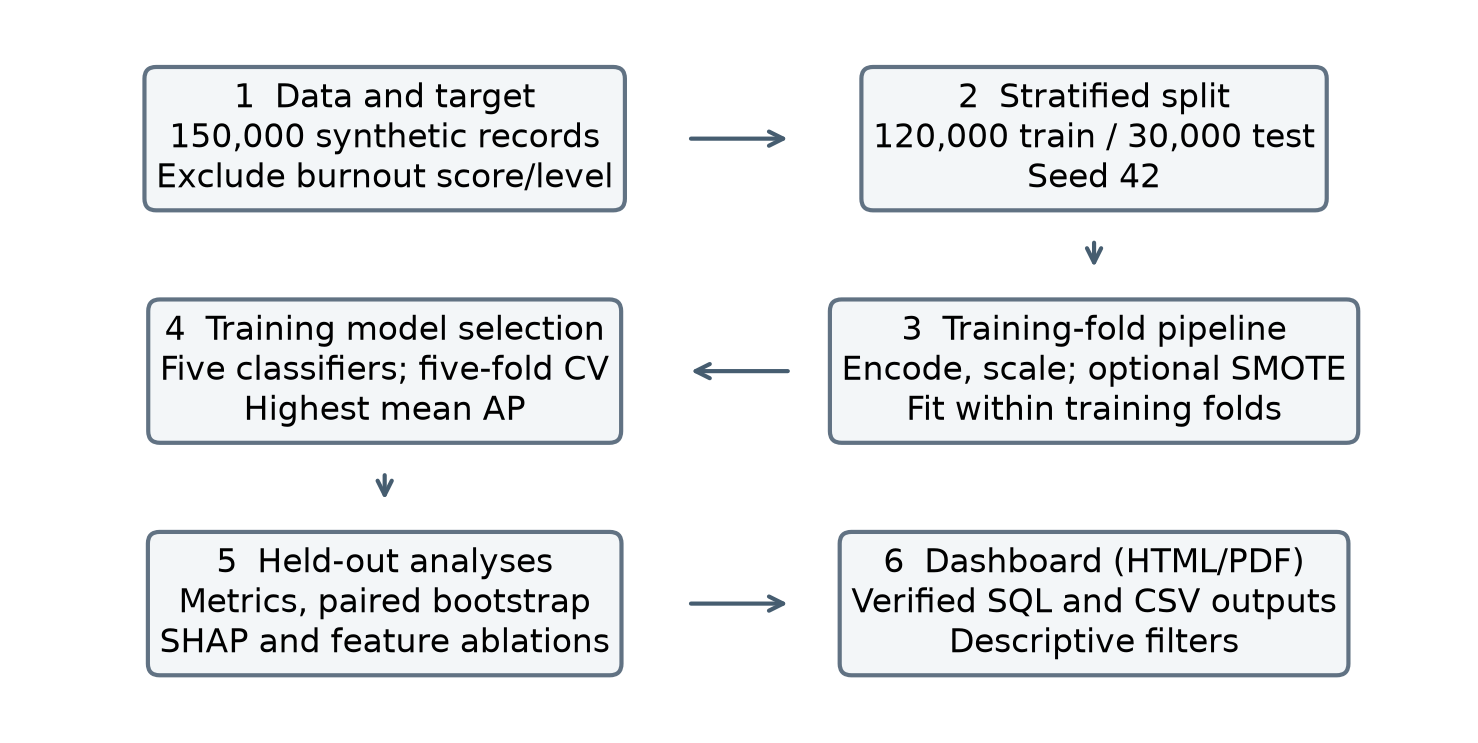
\includegraphics[width=1.0\textwidth]{figures/pipeline_compact.png}\caption{Implemented evaluation workflow; preprocessing and SMOTE fit only training folds.}\label{fig:pipeline}\end{figure}


\subsection{Model configurations}
The comparison includes Logistic Regression, Random Forest \cite{rf}, XGBoost \cite{xgb}, LightGBM \cite{lgb} and a multilayer perceptron (MLP), implemented as scikit-learn-compatible pipelines \cite{sklearn}. Each uses the fixed hyperparameters in Table~\ref{tab:params}, without random-search tuning. The accompanying JSON records fitted-estimator defaults for four models and the archived training arguments for XGBoost, whose native tree file does not retain every training setting. MLP serves as an unweighted log-loss reference with early stopping. Although weighting is technically possible, it was not included in this configuration, so the comparison evaluates the specified pipelines rather than isolating architectural effects under identical objectives. A separate Logistic Regression experiment compares no correction, class weights and SMOTE \cite{smote}.

\begin{table}[!htbp]\caption{Configured hyperparameters. JSON includes fitted defaults for four models and archived XGBoost training kwargs.}\label{tab:params}\centering\small\begin{tabular}{>{\raggedright\arraybackslash}p{.23\textwidth}>{\raggedright\arraybackslash}p{.72\textwidth}}\toprule Model & Configuration \\ \midrule
Logistic Regression & $C=1$, L2, lbfgs, tolerance $10^{-4}$, max\_iter=2000, balanced weights. \\
Random Forest & 300 trees, depth 8, min\_leaf=50, sqrt features, gini, bootstrap, balanced\_subsample, seed 42. \\
XGBoost & 300 trees, depth 3, rate 0.05, row/column sample 0.8, lambda=5, min\_child\_weight=10, binary:logistic, logloss, positive weight 7.1610, seed 42. \\
LightGBM & 300 trees, 8 leaves, rate 0.05, lambda=5, min\_child\_samples=200, row/column sample 0.8, subsample\_freq=1, positive weight 7.1610, seed 42. \\
MLP & (64,32), ReLU, Adam, rate 0.001, alpha=0.001, batch 200, max\_iter=100, early stopping, validation 0.1, patience 10, tolerance $10^{-4}$, seed 42; unweighted. \\
\bottomrule\end{tabular}\end{table}


\subsection{Evaluation and uncertainty}
Model selection uses the highest mean AP from shuffled, stratified five-fold training CV with seed 42. AP is calculated using scikit-learn's non-interpolated definition in Equation~\eqref{eq:ap},
\begin{equation}\mathrm{AP}=\sum_n(R_n-R_{n-1})P_n,\label{eq:ap}\end{equation}
where $P_n$ and $R_n$ denote precision and recall at successive operating points ordered by increasing recall. Equation~\eqref{eq:ap} weights precision by the change in recall and differs from trapezoidal integration of the precision--recall curve. We retain ``PR-AUC'' as the source report's name for AP. The expected random-ranking reference is approximately the positive prevalence, 0.1225, whereas always predicting the majority class gives 87.75\% accuracy. AP therefore provides a more useful primary measure for this imbalanced task \cite{saito}. We also report ROC-AUC and At Risk precision, recall and F1 at threshold 0.5. Training out-of-fold (OOF) probabilities are used to choose an F1-optimal threshold and a threshold targeting recall of at least 80\%, both fixed before test evaluation.

To estimate uncertainty, we calculate percentile 95\% intervals from 2,000 ordinary test-row bootstrap resamples with seed 43. Each resample uses the same sampled rows across models and feature sets, producing paired intervals for AP differences. The multiplicity-weighted AP calculation is checked against literal row resampling, including tied scores. These intervals describe variation conditional on the fitted models and synthetic test distribution; they exclude uncertainty from retraining, model selection and transfer to external populations. The model contrasts are descriptive and have no multiplicity correction.

The exact two-sided Wilcoxon signed-rank comparisons on five nonzero fold pairs all return $p=0.0625$, the smallest attainable exact two-sided p-value for five pairs. This design cannot reject at 0.05, and overlapping training folds make the comparisons dependent. We retain the fold summaries for reproducibility without interpreting the tests as evidence of superiority or equivalence.

\subsection{Model explanation and reproducibility}
We explain the selected Logistic Regression using SHapley Additive exPlanations (SHAP) \cite{shap} on 2,000 test records sampled with seed 42. The values use log-odds units, the natural logarithm of the odds of the At Risk class. The Independent masker retains 100 records from a candidate background of 1,000 training records; the training script explicitly sets \path{max_samples=100}. Equation~\eqref{eq:grouped} combines the encoded contributions for each original variable $j$,
\begin{equation}\Phi_{ij}=\sum_{k\in G_j}\phi_{ik},\label{eq:grouped}\end{equation}
where $i$ identifies a record, $G_j$ contains the encoded columns for variable $j$, and $\phi_{ik}$ is the signed SHAP contribution of encoded column $k$. We then calculate global importance $I_j$ over the $m=2{,}000$ explained records using Equation~\eqref{eq:importance},
\begin{equation}I_j=\frac{1}{m}\sum_{i=1}^{m}|\Phi_{ij}|.\label{eq:importance}\end{equation}
Taking the absolute value in Equation~\eqref{eq:importance} after the signed sum in Equation~\eqref{eq:grouped} allows opposing dummy contributions to cancel within each record. Adding their magnitudes first would count those opposing effects as importance. The regrouped values preserve local log-odds additivity, which we check independently against the linear-model formula. They regroup the existing attributions rather than estimate a new conditional Shapley game. Category shares are normalized sums of $I_j$. We also measure permutation importance as the AP drop on 10,000 test records over five repeats, applying the same row permutation jointly to all columns of a category. Correlated predictors can affect the result, and the drops are neither additive components nor causal effects.

The reproducibility package verifies the five benchmark models against saved CV, OOF and test predictions. The feature-set analysis comprises 30 Logistic Regression fits: one full-training fit and five fold fits for each of F1--F5. F4 and F5 are post hoc sensitivity analyses on the existing hold-out set. Reproduction materials include code, library versions, hyperparameters, row indices, predictions, bootstrap replicates and SQL checks, with commands in \path{README.md}. The native XGBoost JSON and saved preprocessor support verification across operating systems.

\FloatBarrier
\section{Results}
\subsection{Descriptive findings}
The At Risk proportion changes little across work modes, ranging from 12.15\% for Onsite to 12.25\% for Hybrid and 12.33\% for Remote. Working hours show a stronger gradient, with rates rising from 2.76\% in the lowest quartile to 27.15\% in the highest. The largest absolute numeric correlations with the target are stress (0.494), depression (0.408), anxiety (0.365), work--life balance ($-0.319$) and weekly hours (0.294). The cross-tabulation in Table~\ref{tab:heat} further shows how risk varies with stress and hours. An exact count finds zero At Risk cases among the 12,749 records with stress below 4, confirming that the four displayed zeros are observed counts rather than small positive rates rounded to 0.0\%.

\begin{table}[!htbp]\caption{At Risk rates by stress $s$ and weekly hours $h$; counts in parentheses, all $n\geq30$.}\label{tab:heat}\centering\small\begin{tabular}{lrrrr}\toprule Stress & $h\leq40$ & $40<h\leq50$ & $50<h\leq60$ & $h>60$ \\ \midrule
$s<4$ & 0.0\% (4,871) & 0.0\% (6,004) & 0.0\% (1,738) & 0.0\% (136) \\
$4\leq s<6$ & 0.0\% (17,214) & 0.6\% (33,766) & 1.9\% (16,608) & 6.1\% (1,928) \\
$6\leq s<8$ & 4.7\% (8,746) & 14.3\% (26,744) & 28.4\% (20,538) & 47.1\% (3,798) \\
$s\geq8$ & 46.9\% (550) & 65.2\% (2,825) & 81.3\% (3,518) & 93.0\% (1,016) \\
\bottomrule\end{tabular}\end{table}


\subsection{Original-variable importance (RQ1)}
Weekly hours, stress, work--life balance and manager support are the leading variables under both explanation methods (Fig.~\ref{fig:importance}), with permutation AP drops of 0.2030, 0.1352, 0.1236 and 0.0765, respectively. In the fitted linear model, higher hours and stress align with higher output, whereas higher balance and manager support align with lower output. Signed grouping gives work-mode importance of 0.0203 log-odds, compared with 0.6395 when dummy magnitudes are summed before grouping. The aggregation choice does not change predicted probabilities or numeric-variable SHAP values.

At category level, Work environment accounts for 55.08\% of signed-grouped attribution magnitude and Psychological variables for 32.16\% (Table~\ref{tab:importance}). Psychological variables produce the largest joint permutation drop, 0.4043, compared with 0.3953 for Work environment. The difference in ranking follows from the quantities being measured: SHAP shares summarize attribution magnitude, while permutation tests the disruption caused by shuffling inputs. The shares should therefore not be read as explained variance or causal effects.

\begin{table}[!htbp]\caption{Category attribution from signed-grouped SHAP and joint permutation; shares are not causal effects.}\label{tab:importance}\centering\small\begin{tabular}{>{\raggedright\arraybackslash}p{.24\textwidth}rr>{\raggedright\arraybackslash}p{.30\textwidth}}\toprule Category & SHAP share & AP drop & Top feature \\ \midrule
Work environment & 55.08\% & 0.3953 & Weekly working hours \\
Lifestyle & 0.77\% & 0.0001 & Screen time hours \\
Psychological & 32.16\% & 0.4043 & Stress level \\
Demographic & 0.48\% & 0.0001 & Gender \\
Treatment & 11.52\% & 0.0405 & Therapy status \\
\bottomrule\end{tabular}\end{table}


\begin{figure}[!htbp]\centering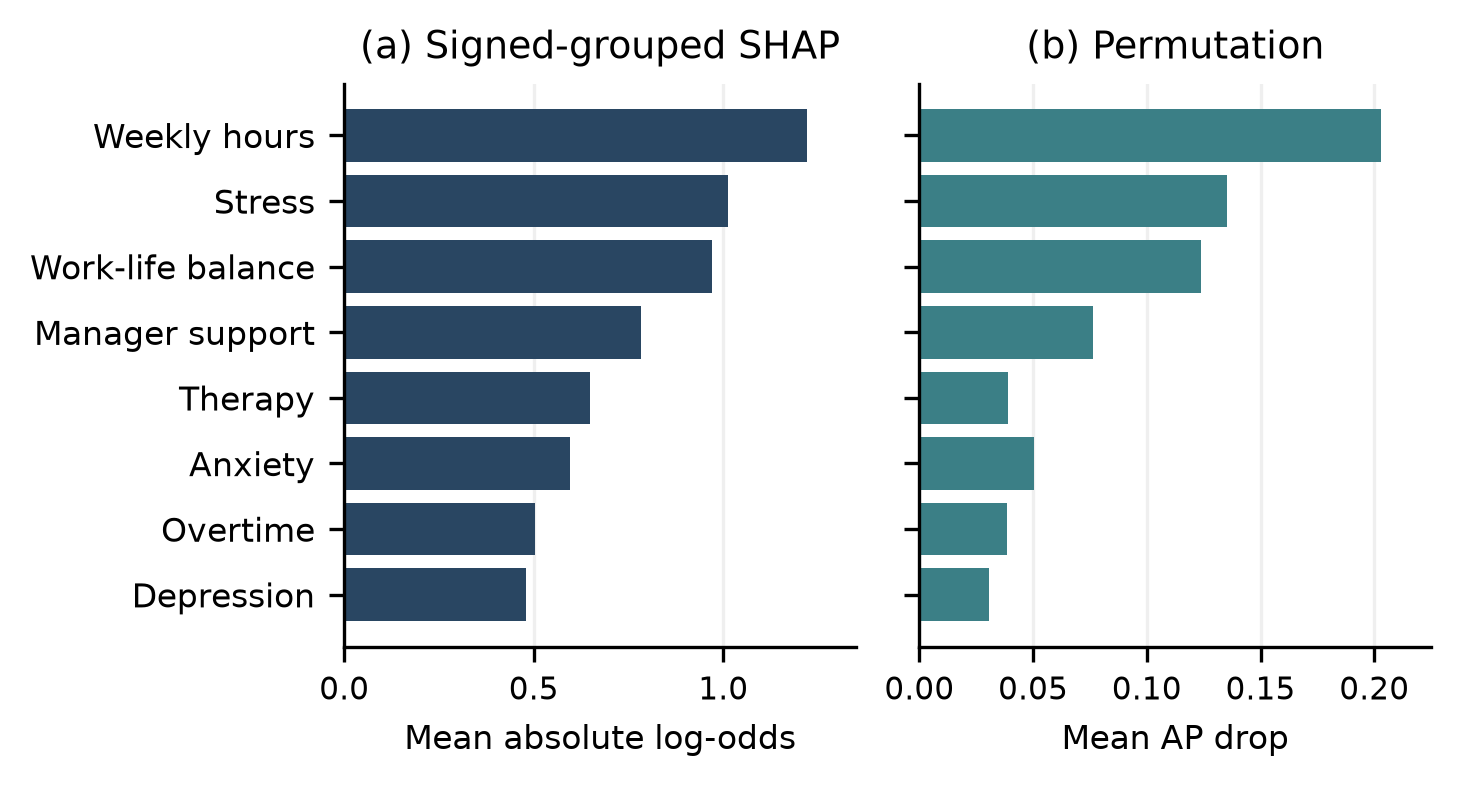
\includegraphics[width=1.0\textwidth]{figures/importance_compact.png}\caption{Original-variable importance: (a) signed-grouped SHAP on 2,000 test records; (b) AP drop on 10,000 test records, five permutations. Shared rows show the eight leading SHAP variables.}\label{fig:importance}\end{figure}


\subsection{Configured model comparison (RQ2)}
Logistic Regression has the highest mean training-CV AP, $0.806\pm0.005$, and is selected for the subsequent analyses. It also achieves the highest test AP, 0.811 (95\% interval 0.800--0.822). This advantage concerns ranking performance: MLP has the highest F1 at the default threshold, 0.710, while Logistic Regression combines higher recall (0.920) with lower precision (0.520). Table~\ref{tab:models} and Fig.~\ref{fig:pr} show these different aspects of performance.

\begin{table}[!htbp]\caption{At Risk test metrics on F1 (23 predictors). Our threshold is 0.5; published settings differ; n/r means not reported.}\label{tab:models}\centering\small\begin{tabular}{>{\raggedright\arraybackslash}p{.32\textwidth}rrrrr}\toprule Model & AP & ROC-AUC & F1 & Prec. & Rec. \\ \midrule
Logistic Regression & 0.811 & 0.964 & 0.664 & 0.520 & 0.920 \\
Random Forest & 0.759 & 0.952 & 0.609 & 0.456 & 0.915 \\
XGBoost & 0.803 & 0.963 & 0.649 & 0.500 & 0.922 \\
LightGBM & 0.803 & 0.963 & 0.650 & 0.501 & 0.925 \\
MLP & 0.807 & 0.963 & 0.710 & 0.748 & 0.675 \\\midrule Patel et al. (XGBoost + SMOTE) & n/r & 0.960 & 0.708 & 0.716 & 0.701 \\
\bottomrule\end{tabular}\end{table}


Relative to Logistic Regression, the paired AP differences and their 95\% intervals are $-0.0518$ ($-0.058$ to $-0.045$) for Random Forest, $-0.0080$ ($-0.010$ to $-0.006$) for XGBoost, $-0.0082$ ($-0.010$ to $-0.006$) for LightGBM and $-0.0043$ ($-0.006$ to $-0.002$) for MLP. These conditional intervals exclude zero, although the smaller differences do not by themselves establish a substantial practical advantage. They also leave the uncertainty from dependent training folds unresolved. Compared with Patel et al., our Logistic Regression has F1 0.664 versus 0.708 and ROC-AUC 0.964 versus 0.960. Since the exact test rows, objectives, preprocessing and thresholds are not matched, these published values provide context rather than a paired significance comparison.

\begin{figure}[!htbp]\centering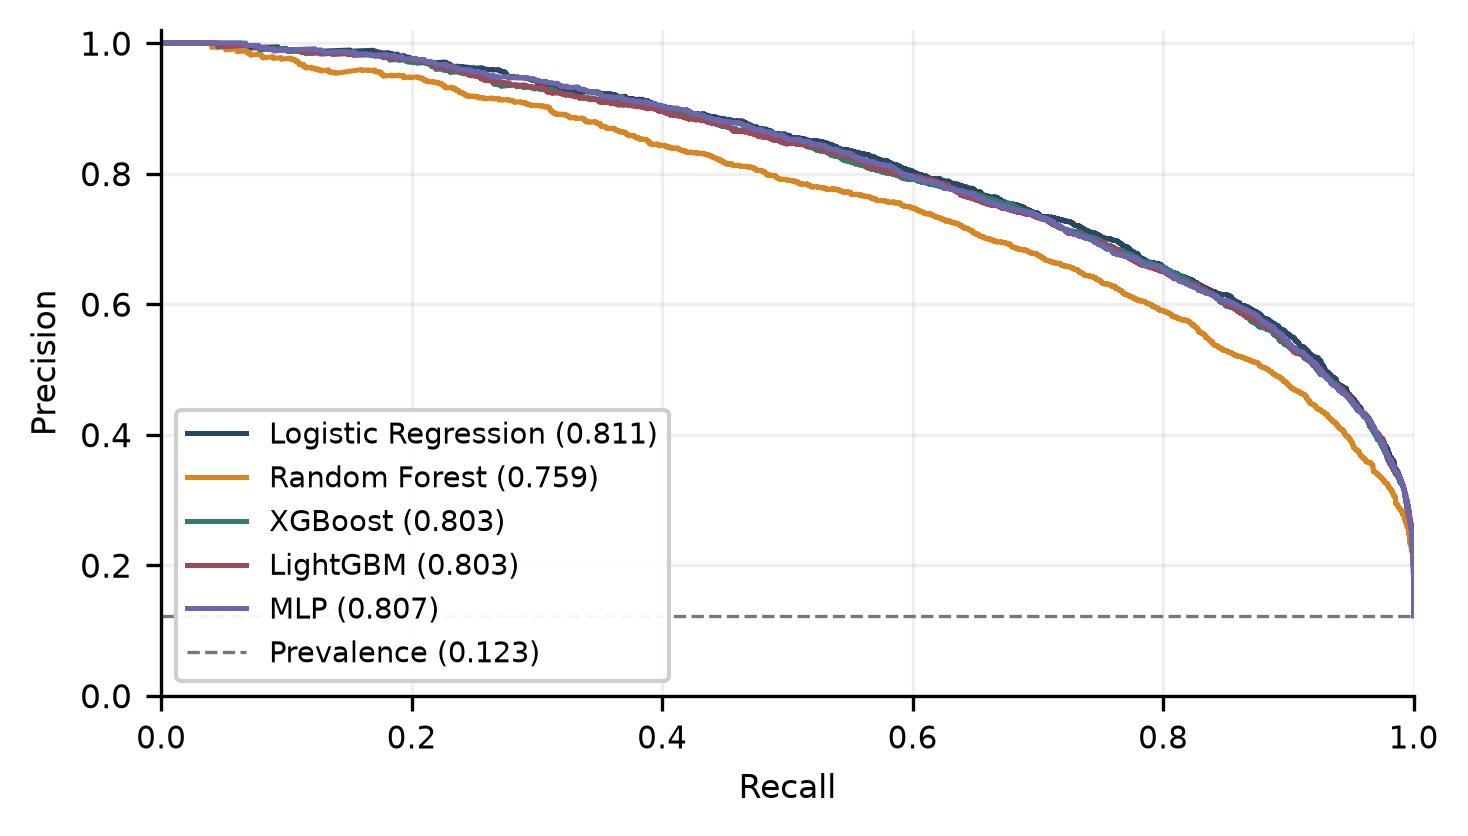
\includegraphics[width=1.0\textwidth]{figures/pr_compact.png}\caption{Precision--recall curves for the five retained fitted models on the fixed test set. Legend values are AP.}\label{fig:pr}\end{figure}


\subsection{Psychological ablation (RQ3) and treatment sensitivities}
Comparing F1 with F2 isolates the removal of the three psychological variables and answers RQ3 (Table~\ref{tab:ablation}). AP falls from 0.810967 to 0.728468, an absolute loss of 0.082499 (95\% paired interval 0.074--0.091), or 10.17\% relative to F1. These differences are calculated from unrounded estimates. F3 removes demographic and treatment variables as well, so its 15.02\% loss cannot be attributed to psychology alone.

\begin{table}[!htbp]\caption{Controlled Logistic Regression ablations. Intervals use 2,000 paired bootstraps; AP loss is F1 minus the row, using unrounded values. F3 and F5 round to the same AP: 0.689199 and 0.689144 before rounding, respectively.}\label{tab:ablation}\centering\small\begin{tabular}{>{\raggedright\arraybackslash}p{.32\textwidth}rrlrr}\toprule Feature set & $p$ & AP & AP 95\% CI & ROC & AP loss \\ \midrule
F1: all features & 23 & 0.811 & [0.800, 0.822] & 0.964 & 0.0000 \\
F2: no psychological & 20 & 0.728 & [0.715, 0.742] & 0.942 & 0.0825 \\
F3: work + lifestyle & 15 & 0.689 & [0.674, 0.704] & 0.932 & 0.1218 \\
F4: no treatment & 21 & 0.790 & [0.778, 0.801] & 0.960 & 0.0211 \\
F5: no psychology/treatment & 18 & 0.689 & [0.674, 0.704] & 0.932 & 0.1218 \\
\bottomrule\end{tabular}\end{table}


Removing treatment alone in F4 gives AP 0.789913 (95\% interval 0.778--0.801), a loss of 0.021054 (0.017--0.025), or 2.60\%. F5 retains demographics while removing psychology and treatment and reaches AP 0.689144, close to F3's 0.689199. The corresponding training-CV AP means and sample standard deviations for F1--F5 are $0.806\pm0.005$, $0.723\pm0.005$, $0.685\pm0.006$, $0.789\pm0.006$ and $0.685\pm0.006$. The results show dependence on treatment information and little additional discrimination from demographics after both information groups are excluded; they do not establish when treatment was recorded or whether either configuration is suitable for deployment.

\subsection{Imbalance, thresholds and dashboard}
In the Logistic Regression comparison, no correction, class weights and SMOTE each give rounded CV AP $0.806\pm0.005$. Their threshold-dependent behaviour differs, however. Class weights increase default-threshold CV recall from 0.637 to 0.911 and reduce precision from 0.770 to 0.516; SMOTE gives recall 0.897 and precision 0.535. At the reported precision, these changes show a shift in the precision--recall trade-off rather than an improvement in AP.

This trade-off is also visible when the threshold is changed. At 0.5, the test set contains 23,199 true negatives, 3,125 false positives, 294 false negatives and 3,382 true positives, totalling 30,000 records. The F1-optimal threshold of 0.8145 selected from training OOF predictions gives test precision 0.706, recall 0.748 and F1 0.727. The recall-target threshold of 0.7383 gives precision 0.650, recall 0.806 and F1 0.720. Both thresholds are chosen from training OOF predictions before test evaluation, so the reported operating points do not result from optimizing test metrics.

The HTML and PDF dashboard brings the model metrics, signed-grouped SHAP and all five ablations together using the same CSV results as the manuscript (Fig.~\ref{fig:dashboard}). Its work-mode filter updates descriptive counts and company-level rates while leaving model scores tied to the fixed test set. The project also includes the full-size dashboard, confusion matrix and threshold plots for closer inspection.

\begin{figure}[!htbp]\centering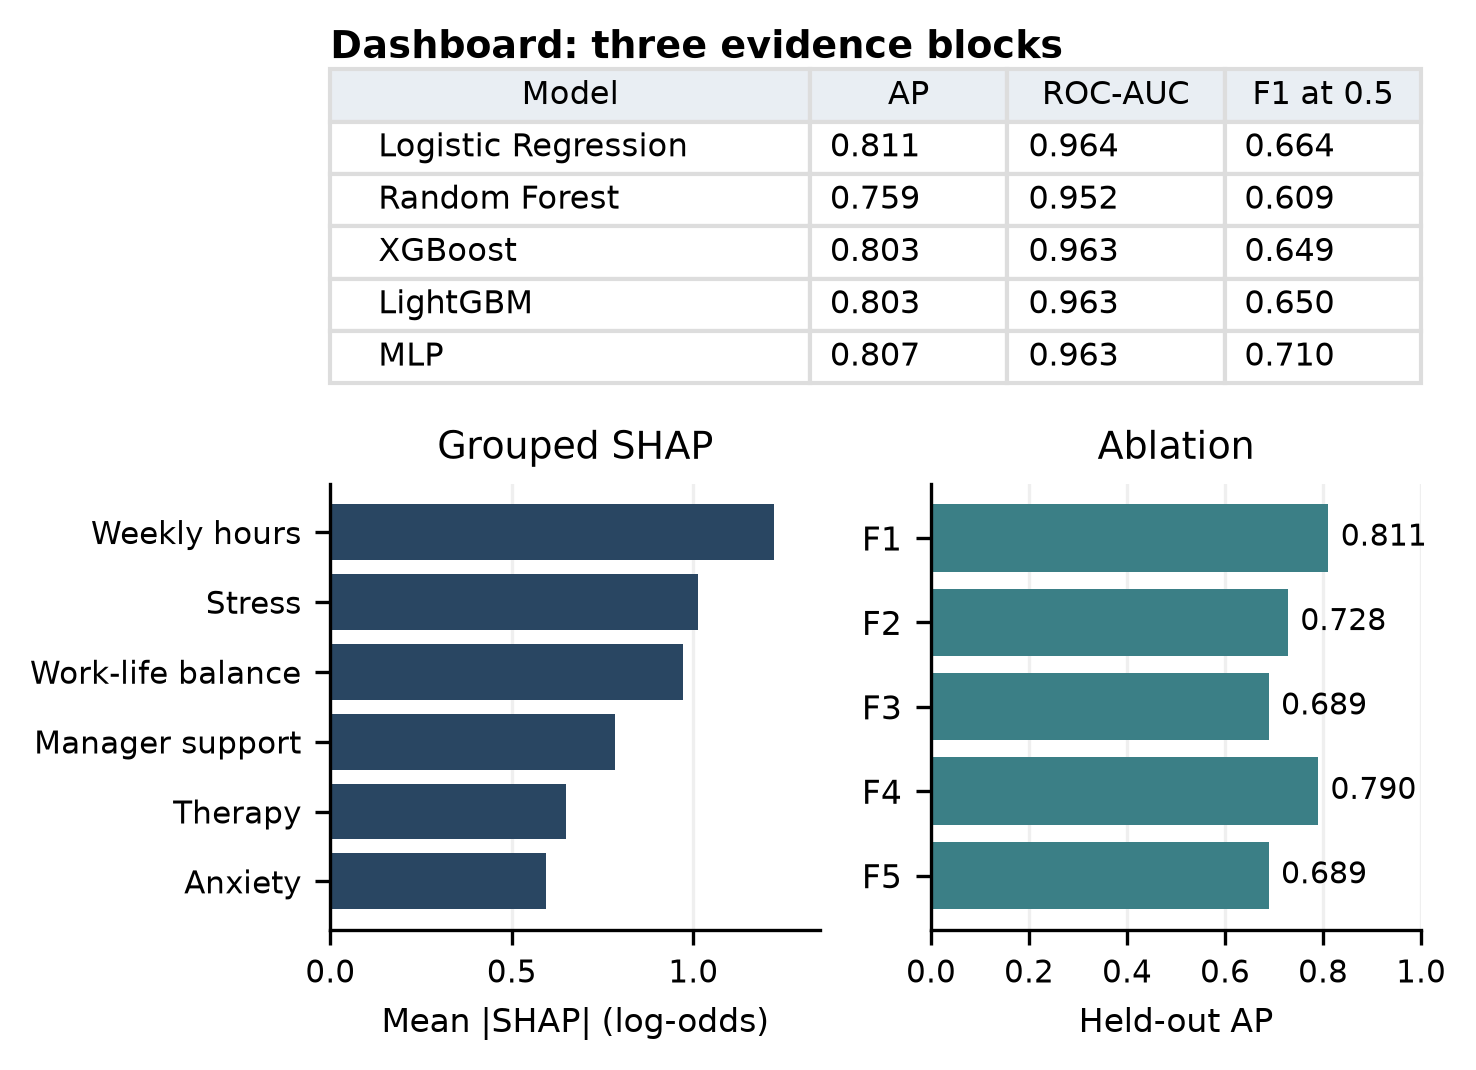
\includegraphics[width=1.0\textwidth]{figures/dashboard_compact.png}\caption{Three-block dashboard: metrics, signed-grouped SHAP and feature ablations F1--F5. Full-size interactive HTML and printable PDF accompany the project.}\label{fig:dashboard}\end{figure}


\FloatBarrier
\section{Discussion}
The absence of At Risk labels among 12,749 low-stress records, together with the gradient at high stress, is consistent with a relatively clean, rule-like process for generating the synthetic labels. At high stress, the At Risk rate rises from 46.9\% among records with no more than 40 weekly hours to 93.0\% above 60 hours. A linear model can rank observations effectively when a small group of variables has such a strong relationship with the label, which offers a plausible explanation for the Logistic Regression result. The associations do not reveal the unavailable generator formula or establish that linear models would perform best in real workplaces.

The comparison of attribution aggregations shows how preprocessing can affect interpretation even when predictions remain unchanged. Summing the magnitudes of opposing one-hot contributions makes work mode appear important despite its nearly constant descriptive risk rates. Signed regrouping removes this inflation, although the resulting values still explain the fitted model under independent masking. The treatment ablation addresses a related concern about which information is available at prediction time. Its nonzero loss shows that treatment indicators contribute to discrimination, but unknown timing prevents a conclusion that they leak the outcome. F4 remains a synthetic, cross-sectional classifier, and stress, anxiety and depression may also overlap conceptually with burnout. Evaluating screening before treatment would require predictors recorded before independently measured outcomes.

The main limitation is the absence of validation on real occupational data, including external, temporal and subgroup evaluation. Combining Moderate and High labels also prevents assessment of severity. The fixed configurations use different weighting objectives, particularly the unweighted MLP, while five-fold comparisons and conditional bootstrap omit uncertainty from retraining and population transfer. SHAP depends on a background of 100 effective records, and the additional sensitivities were examined retrospectively on the existing test set. Future work should therefore use representative timestamped data with validated outcomes, assess calibration and subgroup performance, and select thresholds according to support capacity and the cost of missed cases. Increasing the number of resamples within this dataset would not resolve those questions.

\FloatBarrier
\section{Conclusion}
Weekly working hours, stress, work--life balance and manager support are the leading variables in this synthetic benchmark. Signed-grouped SHAP gives Work environment and Psychological attribution shares of 55.08\% and 32.16\%. Logistic Regression, selected by training CV, achieves test AP 0.811 (95\% interval 0.800--0.822), ROC-AUC 0.964 and F1 0.664 with all predictors in F1. Removing only the psychological variables lowers AP by 0.0825 to 0.728. Treatment-excluded F4 achieves AP 0.790 (95\% interval 0.778--0.801) and is the recommended benchmark configuration when treatment timing is unknown. Retaining only work environment and lifestyle gives AP 0.689. These comparisons answer the research questions within the simulated records; F4 and the other configurations still require temporal and external validation before any screening application.

\section*{Data and Code Availability}
The dataset is available from Kaggle under CC0: Public Domain \cite{dataset}. Analysis code, library versions, model artifacts, row indices, predictions, SQL checks and reproduction instructions are available at \url{https://github.com/Group15-FA26-AI2109/burnout-risk-classification}, with commands in \path{README.md}.


\begin{thebibliography}{99}
\bibitem{who} World Health Organization: Burn-out an occupational phenomenon: International Classification of Diseases (2019). \url{https://www.who.int/news/item/28-05-2019-burn-out-an-occupational-phenomenon-international-classification-of-diseases}. Accessed 19 October 2026.
\bibitem{wellness} Developer Nation: State of Developer Wellness Report 2024. Industry survey report (2024). \url{https://developernation.net/resources/reports/state-of-developer-wellness-report-2024/}. Accessed 27 October 2026.
\bibitem{padmashali} Padmashali, A.: Prevalence of stress and burnout among information technology professionals during COVID-19 pandemic due to work from home situation. International Journal of Community Medicine and Public Health 10(4), 1530--1536 (2023). \url{https://doi.org/10.18203/2394-6040.ijcmph20230936}.
\bibitem{trink23} Trinkenreich, B., Stol, K.-J., Steinmacher, I., Gerosa, M., Sarma, A., Lara, M., Feathers, M., Ross, N., Bishop, K.: A model for understanding and reducing developer burnout. In: ICSE Software Engineering in Practice (2023). \url{https://doi.org/10.1109/ICSE-SEIP58684.2023.00010}.
\bibitem{trink24} Trinkenreich, B., Santos, F., Stol, K.-J.: Predicting attrition among software professionals: antecedents and consequences of burnout and engagement. ACM Trans. Softw. Eng. Methodol. 33(8), 218:1--218:45 (2024). \url{https://doi.org/10.1145/3691629}.
\bibitem{mapping} Tulili, T.R., Capiluppi, A., Rastogi, A.: Burnout in software engineering: a systematic mapping study. Information and Software Technology 155, 107116 (2023). \url{https://doi.org/10.1016/j.infsof.2022.107116}.
\bibitem{review} Tulili, T.R., Rastogi, A., Capiluppi, A.: Machine learning models for the early detection of burnout in software engineering: a systematic literature review. arXiv:2603.23063v1 (2026). \url{https://doi.org/10.48550/arXiv.2603.23063}.
\bibitem{feng} Feng, Z., Afroz, S., Sarma, A.: From gains to strains: modeling developer burnout with GenAI adoption. In: Proceedings of the IEEE/ACM 48th International Conference on Software Engineering (ICSE-SEIS), pp. 125--136. ACM (2026). \url{https://doi.org/10.1145/3786581.3786934}.
\bibitem{ribeiro} Ribeiro, D.M.: Understanding the relationships between the perceptions of burnout and instability in software engineering. In: Proceedings of the XXXVI Brazilian Symposium on Software Engineering, pp. 58--67. ACM (2022). \url{https://doi.org/10.1145/3555228.3555251}.
\bibitem{michels} Michels, L.-M., Petkova, A., Richter, M., Farley, A., Graziotin, D., Wagner, S.: Overwhelmed software developers. IEEE Software 41(4), 51--59 (2024). \url{https://doi.org/10.1109/MS.2024.3374821}.
\bibitem{un} United Nations, Department of Economic and Social Affairs: Goal 3: Ensure healthy lives and promote well-being for all at all ages. Target 3.4 (n.d.). \url{https://sdgs.un.org/goals/goal3}. Accessed 19 October 2026.
\bibitem{patel} Patel, T., Sharma, G., Sarangi, P.K., Saxena, M., Dobariya, A., Ionescu, V.M., Bizon, N.: Feature attribution dynamics under imbalanced learning algorithms: an explainable machine learning framework for burnout risk prediction. Algorithms 19(9), 716 (2026). \url{https://doi.org/10.3390/a19090716}.
\bibitem{adapa} Adapa, K., Pillai, M., Foster, M., Charguia, N., Mazur, L.: Using explainable supervised machine learning to predict burnout in healthcare professionals. Studies in Health Technology and Informatics 294, 58--62 (2022). \url{https://doi.org/10.3233/SHTI220396}.
\bibitem{dataset} Gupta, S.: Employee Mental Health \& Burnout Dataset. Kaggle, version 1, released 15 March 2026 (2026). \url{https://www.kaggle.com/datasets/suhanigupta04/employee-mental-health-and-burnout-dataset}. Accessed 27 October 2026.
\bibitem{rf} Breiman, L.: Random forests. Machine Learning 45(1), 5--32 (2001).
\bibitem{xgb} Chen, T., Guestrin, C.: XGBoost: a scalable tree boosting system. In: ACM SIGKDD, pp. 785--794 (2016).
\bibitem{lgb} Ke, G., et al.: LightGBM: a highly efficient gradient boosting decision tree. In: Advances in Neural Information Processing Systems 30, 3146--3154 (2017).
\bibitem{sklearn} Pedregosa, F., et al.: Scikit-learn: machine learning in Python. Journal of Machine Learning Research 12, 2825--2830 (2011).
\bibitem{smote} Chawla, N.V., Bowyer, K.W., Hall, L.O., Kegelmeyer, W.P.: SMOTE: synthetic minority over-sampling technique. Journal of Artificial Intelligence Research 16, 321--357 (2002).
\bibitem{saito} Saito, T., Rehmsmeier, M.: The precision-recall plot is more informative than the ROC plot when evaluating binary classifiers on imbalanced datasets. PLoS ONE 10(3), e0118432 (2015).
\bibitem{shap} Lundberg, S.M., Lee, S.-I.: A unified approach to interpreting model predictions. In: Advances in Neural Information Processing Systems 30, 4765--4774 (2017).
\end{thebibliography}\end{document}